% ─────────────────────────────────────────────────────────────────────────────
% back/annexes.tex — Annexes A through E
% ─────────────────────────────────────────────────────────────────────────────

\appendix
\renewcommand{\chaptername}{Annexe}

% ─────────────────────────────────────────────────────────────────────────────
\chapter{UML Diagrams}
\label{annexe:uml}
% ─────────────────────────────────────────────────────────────────────────────

This annexe contains the full set of UML diagrams produced during the analysis and design phase of the project. The diagrams presented in the main body of the mémoire (Chapter~2) are condensed versions intended to fit within the page layout; the diagrams here show the complete models.

\bigskip
\noindent\textbf{Figure A.1} — Complete use case diagram including all actors, all use cases, and actor generalisation relationships.

\begin{figure}[H]
\centering
\begin{tikzpicture}[
  actor/.style={rectangle, draw=black!60, fill=gray!10, rounded corners=3pt,
                minimum width=2.4cm, minimum height=0.6cm, align=center, font=\scriptsize\bfseries},
  uc/.style={ellipse, draw=black!70, fill=blue!5, minimum width=4.5cm, minimum height=0.72cm,
             align=center, font=\scriptsize},
  ucadm/.style={ellipse, draw=black!70, fill=orange!8, minimum width=4.5cm, minimum height=0.72cm,
                align=center, font=\scriptsize},
  sys/.style={rectangle, draw=black!50, dashed, rounded corners=5pt, inner sep=8pt},
  assoc/.style={thick, black!50},
  gen/.style={thick, black!70, -{Triangle[open, length=5pt, width=5pt]}}
]
  \node[sys, minimum width=11cm, minimum height=13.8cm] (sys) at (5.5,-6.8) {};
  \node[font=\scriptsize\bfseries, anchor=north west] at (sys.north west) {\textit{Mobile Match Algeria — System Boundary}};

  % Use cases accessible by all users (visitor + registered + admin)
  \node[uc] (uc1) at (5.5,-0.7) {Browse \& Filter Offers};
  \node[uc] (uc2) at (5.5,-1.9) {View Offer Details};
  \node[uc] (uc3) at (5.5,-3.1) {Compare Plans (side-by-side)};
  % Use cases for registered users and admin
  \node[uc] (uc4) at (5.5,-4.4) {Get Personalised Recommendations};
  \node[uc] (uc5) at (5.5,-5.6) {Save / Unsave a Plan};
  \node[uc] (uc6) at (5.5,-6.8) {View Saved Plans};
  \node[uc] (uc7) at (5.5,-8.0) {Edit Usage Profile};
  \node[uc] (uc8) at (5.5,-9.2) {View \& Manage Notifications};
  % Admin-only use cases
  \node[ucadm] (uc9)  at (5.5,-10.5) {Trigger Scrape Run};
  \node[ucadm] (uc10) at (5.5,-11.8) {View Scrape Logs \& Statistics};
  \node[ucadm] (uc11) at (5.5,-13.0) {View \& Manage Notifications};

  % Actors (left side)
  \node[actor] (visitor) at (-0.5,-1.3) {Visitor};
  \node[actor] (user)    at (-0.5,-6.8) {Registered\\User};
  \node[actor] (admin)   at (-0.5,-11.8) {Administrator};

  % Generalisation arrows (open triangle = is-a / inherits; no label in UML)
  \draw[gen] (user.north)  -- (visitor.south);
  \draw[gen] (admin.north) -- (user.south);

  % Visitor associations
  \draw[assoc] (visitor.east) -- (uc1.west);
  \draw[assoc] (visitor.east) -- (uc2.west);
  \draw[assoc] (visitor.east) -- (uc3.west);

  % Registered User additional associations
  \draw[assoc] (user.east) -- (uc4.west);
  \draw[assoc] (user.east) -- (uc5.west);
  \draw[assoc] (user.east) -- (uc6.west);
  \draw[assoc] (user.east) -- (uc7.west);
  \draw[assoc] (user.east) -- (uc8.west);

  % Admin additional (exclusive) associations
  \draw[assoc] (admin.east) -- (uc9.west);
  \draw[assoc] (admin.east) -- (uc10.west);
  \draw[assoc] (admin.east) -- (uc11.west);
\end{tikzpicture}
\caption{Complete use case diagram --- actor generalisation and all use cases}
\label{fig:usecase-full}
\end{figure}

\noindent\textbf{Figure A.2} — Class diagram showing all model classes, their attributes, and their associations.

\begin{figure}[H]
\centering
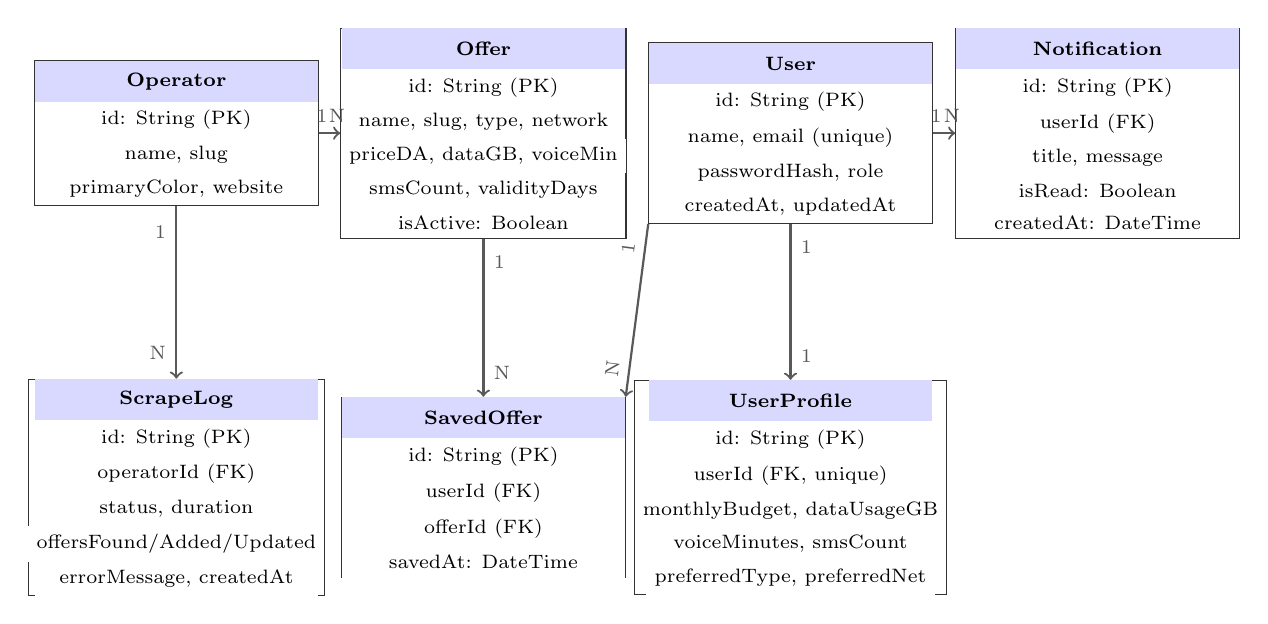
\begin{tikzpicture}[
  cls/.style={rectangle, draw=black!80, fill=white, align=left, font=\scriptsize, inner sep=0pt},
  hdr/.style={fill=blue!15, font=\scriptsize\bfseries, align=center, minimum height=0.52cm, minimum width=3.6cm},
  row/.style={fill=white, minimum height=0.40cm, minimum width=3.6cm, align=left, inner sep=3pt},
  assoc/.style={thick, ->, black!65}
]
  %% ── Row 1: Operator · Offer · User · Notification ─────────────────────────
  \matrix[cls, ampersand replacement=\&] (op) at (0,0) {
    \node[hdr]{Operator}; \\
    \node[row]{id: String (PK)}; \\
    \node[row]{name, slug}; \\
    \node[row]{primaryColor, website}; \\
  };
  \matrix[cls, ampersand replacement=\&] (offer) at (3.9,0) {
    \node[hdr]{Offer}; \\
    \node[row]{id: String (PK)}; \\
    \node[row]{name, slug, type, network}; \\
    \node[row]{priceDA, dataGB, voiceMin}; \\
    \node[row]{smsCount, validityDays}; \\
    \node[row]{isActive: Boolean}; \\
  };
  \matrix[cls, ampersand replacement=\&] (user) at (7.8,0) {
    \node[hdr]{User}; \\
    \node[row]{id: String (PK)}; \\
    \node[row]{name, email (unique)}; \\
    \node[row]{passwordHash, role}; \\
    \node[row]{createdAt, updatedAt}; \\
  };
  \matrix[cls, ampersand replacement=\&] (notif) at (11.7,0) {
    \node[hdr]{Notification}; \\
    \node[row]{id: String (PK)}; \\
    \node[row]{userId (FK)}; \\
    \node[row]{title, message}; \\
    \node[row]{isRead: Boolean}; \\
    \node[row]{createdAt: DateTime}; \\
  };

  %% ── Row 2: ScrapeLog · SavedOffer · UserProfile ───────────────────────────
  \matrix[cls, ampersand replacement=\&] (scrape) at (0,-4.5) {
    \node[hdr]{ScrapeLog}; \\
    \node[row]{id: String (PK)}; \\
    \node[row]{operatorId (FK)}; \\
    \node[row]{status, duration}; \\
    \node[row]{offersFound/Added/Updated}; \\
    \node[row]{errorMessage, createdAt}; \\
  };
  \matrix[cls, ampersand replacement=\&] (saved) at (3.9,-4.5) {
    \node[hdr]{SavedOffer}; \\
    \node[row]{id: String (PK)}; \\
    \node[row]{userId (FK)}; \\
    \node[row]{offerId (FK)}; \\
    \node[row]{savedAt: DateTime}; \\
  };
  \matrix[cls, ampersand replacement=\&] (profile) at (7.8,-4.5) {
    \node[hdr]{UserProfile}; \\
    \node[row]{id: String (PK)}; \\
    \node[row]{userId (FK, unique)}; \\
    \node[row]{monthlyBudget, dataUsageGB}; \\
    \node[row]{voiceMinutes, smsCount}; \\
    \node[row]{preferredType, preferredNet}; \\
  };

  %% ── Associations ──────────────────────────────────────────────────────────
  % Operator → Offer  (1 to N)
  \draw[assoc] (op.east) --
    node[above, font=\scriptsize, pos=0.15]{1}
    node[above, font=\scriptsize, pos=0.85]{N}
    (offer.west);
  % Operator → ScrapeLog  (1 to N)
  \draw[assoc] (op.south) --
    node[left, font=\scriptsize, pos=0.15]{1}
    node[left, font=\scriptsize, pos=0.85]{N}
    (scrape.north);
  % Offer → SavedOffer  (1 to N)
  \draw[assoc] (offer.south) --
    node[right, font=\scriptsize, pos=0.15]{1}
    node[right, font=\scriptsize, pos=0.85]{N}
    (saved.north);
  % User → SavedOffer  (1 to N) — diagonal, does not cross Offer→SavedOffer
  \draw[assoc] (user.south west) --
    node[above, sloped, font=\scriptsize, pos=0.15]{1}
    node[above, sloped, font=\scriptsize, pos=0.85]{N}
    (saved.north east);
  % User → UserProfile  (1 to 1)
  \draw[assoc] (user.south) --
    node[right, font=\scriptsize, pos=0.15]{1}
    node[right, font=\scriptsize, pos=0.85]{1}
    (profile.north);
  % User → Notification  (1 to N) — horizontal, no overlap
  \draw[assoc] (user.east) --
    node[above, font=\scriptsize, pos=0.15]{1}
    node[above, font=\scriptsize, pos=0.85]{N}
    (notif.west);
\end{tikzpicture}
\caption{Class diagram of the Mobile Match Algeria data model}
\label{fig:class-diagram}
\end{figure}

\noindent\textbf{Figure A.3} — Sequence diagram for the user registration and login flow.

\begin{figure}[H]
\centering
\begin{tikzpicture}[
  actor/.style={rectangle, draw=black!70, fill=gray!15, minimum width=3cm,
                minimum height=0.55cm, align=center, font=\small\bfseries},
  msg/.style={-{Stealth[length=4pt]}, thick},
  retmsg/.style={-{Stealth[length=4pt]}, thick, dashed},
  note/.style={font=\scriptsize, fill=yellow!20, draw=gray!60,
               rounded corners=2pt, inner sep=3pt, align=left}
]
  \node[actor] (client) at (0,0)    {Browser};
  \node[actor] (api)    at (5.5,0)  {NextAuth API};
  \node[actor] (db)     at (11,0)   {Database};

  \foreach \x in {0,5.5,11} \draw[gray!50, thick] (\x,-0.35) -- (\x,-11.0);

  %% ── Registration ──────────────────────────────────────────────────────────
  \node[font=\small\bfseries, gray!70] at (-2.4,-0.9) {Register};
  \draw[msg]    (0,-1.1)  -- (5.5,-1.1)
    node[midway, above, font=\scriptsize]{POST /api/auth/register \{name, email, password\}};
  \draw[msg]    (5.5,-2.0) -- (11,-2.0)
    node[midway, above, font=\scriptsize]{SELECT: check email uniqueness};
  \draw[retmsg] (11,-2.7)  -- (5.5,-2.7)
    node[midway, above, font=\scriptsize]{Not found — OK};
  \node[note, anchor=west] at (5.8,-3.5)  {Hash password (bcrypt, cost=12)};
  \draw[msg]    (5.5,-4.3) -- (11,-4.3)
    node[midway, above, font=\scriptsize]{INSERT User \{name, email, passwordHash\}};
  \draw[retmsg] (5.5,-5.1) -- (0,-5.1)
    node[midway, above, font=\scriptsize]{201 Created — redirect to /login};

  %% ── Separator ─────────────────────────────────────────────────────────────
  \draw[dashed, gray!60] (-1.0,-5.8) -- (12.0,-5.8);

  %% ── Login ─────────────────────────────────────────────────────────────────
  \node[font=\small\bfseries, gray!70] at (-2.4,-6.4) {Login};
  \draw[msg]    (0,-6.6)   -- (5.5,-6.6)
    node[midway, above, font=\scriptsize]{POST /api/auth/signin \{email, password\}};
  \draw[msg]    (5.5,-7.5) -- (11,-7.5)
    node[midway, above, font=\scriptsize]{SELECT User WHERE email = ?};
  \draw[retmsg] (11,-8.2)  -- (5.5,-8.2)
    node[midway, above, font=\scriptsize]{User record + passwordHash};
  \node[note, anchor=west] at (5.8,-9.0)  {bcrypt.compare(password, hash)};
  \node[note, anchor=west] at (5.8,-9.7)  {Sign JWT \{role, id, secret\}};
  \draw[retmsg] (5.5,-10.5) -- (0,-10.5)
    node[midway, above, font=\scriptsize]{200 OK + Set-Cookie: session JWT};
  \node[note, anchor=west] at (0.3,-11.2) {Redirect to /offers};
\end{tikzpicture}
\caption{Sequence diagram --- user registration and login flow}
\label{fig:seq-auth}
\end{figure}

% ─────────────────────────────────────────────────────────────────────────────
\chapter{Data Model Summary}
\label{annexe:schema}
% ─────────────────────────────────────────────────────────────────────────────

The data model is defined in \texttt{prisma/schema.prisma} using the Prisma schema language. It consists of seven application-defined entities whose primary fields and relations are summarised in Table~\ref{tab:schema-entities}. Authentication infrastructure models managed by NextAuth.js (\texttt{Account}, \texttt{Session}) are excluded from this summary. The full schema file is available in the project repository.

\begin{table}[H]
  \caption{Prisma schema entities and primary fields}
  \label{tab:schema-entities}
  \centering\small
  \begin{tabular}{|p{2.4cm}|p{7.5cm}|p{3.5cm}|}
    \hline
    \textbf{Entity} & \textbf{Key fields} & \textbf{Relations} \\
    \hline
    User         & id, name, email, role, passwordHash, createdAt & SavedOffer, Notification, UserProfile \\
    \hline
    UserProfile  & id, userId, monthlyBudget, dataUsageGB, voiceMinutes, preferredType & User \\
    \hline
    Offer        & id, operator, name, type, priceDA, dataGB, voiceMinutes, validityDays, isActive & SavedOffer \\
    \hline
    SavedOffer   & id, userId, offerId, savedAt & User, Offer \\
    \hline
    Notification & id, userId, title, message, type, isRead, createdAt & User \\
    \hline
    ScrapeLog    & id, operatorId, status, offersFound, offersAdded, offersUpdated, duration, startedAt & Operator \\
    \hline
    Operator     & id, name, slug, logoUrl, websiteUrl, primaryColor & Offer, ScrapeLog \\
    \hline
  \end{tabular}
\end{table}


